\section{问题三：预报更新下的滚动随机规划}
\subsection{建模思路与信息边界}
问题三在问题二的日前计划基础上，增加了光伏预报更新与购电合同调整机制。本文将31天历史场景与滚动时域优化结合：0:00利用最新光伏预报制定全天计划；6:00、12:00等更新时刻重新构造剩余时段的净负荷场景，在已执行储能状态和已确认合同的基础上调整未来策略。实际净负荷超出计划净供能的部分，仍由五倍电价紧急购电补足。

将一天按记录顺序划分为144个十分钟时段，$\Delta t=1/6\,\mathrm h$；内部索引$t=1,\ldots,144$，预报时刻$r\in\{0,6,12,18\}$对应已完成时段数$\tau_r=6r$。设$\mathcal T_r=\{\tau_r+1,\ldots,144\}$。每次优化只使用前31天的历史实际数据、当次已发布预报，以及发布前最后一个已完成时段的观测值。目标日未来实际负载和光伏仅用于事后评价，不进入当次决策。

本文延续问题二每日首末储电量为6000 kWh的周期边界，只使用预报中截至当日24:00的部分。日内更新时，初始储电量必须承接已经执行的充放电结果，不能在6:00或12:00重新设为6000 kWh。该边界有利于比较不同预报组合，但限制了跨日储能和次日预报信息的利用。

\subsection{光伏预报插值及净负荷场景}
附件3按每天四个发布时间给出未来24小时整点预报。设$\widehat P_{d,r,h}$为第$d$日$r$时发布的第$h$小时光伏功率预报，令$y_0$为当前已观测光伏功率，$y_h=\widehat P_{d,r,h}$。0:00锚点取零，其他时刻使用发布前最后一条实际记录。对相邻整点间的$x\in[h,h+1]$，线性插值为
\begin{equation}
\widetilde P_{d,r}(x)=(h+1-x)y_h+(x-h)y_{h+1}.
\end{equation}
本文在十分钟区间中点采样，$\widehat P^{10}_{d,r,t}=\widetilde P_{d,r}((t-\tau_r-1/2)\Delta t)$。历史预测误差采用相同插值方式计算，保证场景、优化和误差评价口径一致。

对历史日期$s\in\mathcal S_d=\{d-31,\ldots,d-1\}$，按相同发布时间和插值方法计算光伏预测误差，并与同一天负载配对：
\begin{align}
e_{s,r,t}&=P^{\mathrm{PV}}_{s,t}-\widehat P^{10}_{s,r,t},\\
P^{\mathrm{PV},(s)}_{d,r,t}&=\max\{0,\widehat P^{10}_{d,r,t}+e_{s,r,t}\},\\
N^{(s)}_{d,r,t}&=\bigl(P^{\mathrm L}_{s,t}-P^{\mathrm{PV},(s)}_{d,r,t}\bigr)\Delta t,
\qquad \pi_s=1/31.\label{eq:p3-scenario}
\end{align}
式\eqref{eq:p3-scenario}以目标日新预报为中心，叠加近期历史误差，避免将预报视为确定值；非负截断避免出现负光伏功率。负载不另行拟合预测模型，同日负载与光伏误差的配对保留历史联合变化。其适用前提是近期误差具有一定可迁移性，尚不能保证极端天气或负载突变均被31个场景覆盖。

\subsection{初始计划与逐次调整结算}
记$G^0_t$为0:00初始合同购电量；日内更新前后的合同量分别为$G^{\mathrm{old}}_t$和$G^{\mathrm{new}}_t$。定义增购量$A^r_t$和削减量$B^r_t$，则
\begin{equation}
G^{\mathrm{new}}_t=G^{\mathrm{old}}_t+A^r_t-B^r_t,
\qquad A^r_t\geq0,\quad 0\leq B^r_t\leq G^{\mathrm{old}}_t.
\label{eq:p3-contract}
\end{equation}
本文将题面50\%违约电价解释为取消电量仅退回原价的50\%，被取消部分承担其余50\%损失。每次调整相对于上一版已确认合同结算，其净费用为
\begin{equation}
K_d^r=\sum_{t\in\mathcal T_r}p_t(1.5A^r_t-0.5B^r_t).
\label{eq:p3-cash}
\end{equation}
例如原计划100 kWh削减为80 kWh，初始支付$100p$，获得$10p$退款，最终支出$90p$；若增至120 kWh，则支付$100p+1.5p\times20=130p$。因此调整净费用可以为负，不能将退款误记为负违约损失，也不能在保留全部初始费用的同时再次对被取消电量重复收费。此处采用交付时段对应的分时电价$p_t$；逐次结算和退款解释均为本文统一的交易口径。

相同时段若同时增购和削减相同电量，会增加$p_t$倍该电量的费用而不改变合同。因此，正电价下同时增减没有经济优势。多次调整的路径仍影响结算，不能只用最终合同与初始合同之差代替每次交易。

\subsection{随机线性规划及滚动执行}
设$C_t,D_t,E_t$分别为充电输入电量、放电输出电量和时段末储电量，$U^{(s)}_t$为场景紧急购电量。0:00的目标为
\begin{equation}
\min\ \sum_{t=1}^{144}p_tG^0_t
+\frac1{31}\sum_{s\in\mathcal S_d}\sum_{t=1}^{144}5p_tU^{(s)}_t
+\varepsilon\sum_{t=1}^{144}(C_t+D_t),\quad\varepsilon=10^{-8}.
\label{eq:p3-init}
\end{equation}
在$r>0$时，已支付合同费用及过去费用为沉没成本，剩余时域的优化目标改为
\begin{equation}
\min\ \sum_{t\in\mathcal T_r}p_t(1.5A^r_t-0.5B^r_t)
+\frac1{31}\sum_s\sum_{t\in\mathcal T_r}5p_tU^{(s)}_t
+\varepsilon\sum_{t\in\mathcal T_r}(C_t+D_t).
\label{eq:p3-roll}
\end{equation}
各阶段满足共同的设备与场景约束：
\begin{align}
U^{(s)}_t&\geq N^{(s)}_{d,r,t}-G_t-D_t+C_t,\qquad U^{(s)}_t\geq0,\\
E_t&=E_{t-1}+0.9C_t-D_t/0.9,\\
1200&\leq E_t\leq10800,\qquad 0\leq C_t,D_t\leq5000\Delta t,\\
G_t&\geq0,\qquad E_{144}=6000,\\
E_{\tau_r}&=E^{\mathrm{exec}}_{\tau_r}.\label{eq:p3-boundary}
\end{align}
0:00取$E^{\mathrm{exec}}_0=6000$，调整阶段另加入式\eqref{eq:p3-contract}。上述不等式等价于在场景电量平衡中引入非负供能富余量后将其消去。每个阶段的合同与充放电变量在31个场景间共享，紧急购电变量随场景变化。目标中的小惩罚仅用于减少不必要的吞吐；报告费用剔除数值辅助惩罚。

求解器显式保留场景供能富余变量，以稀疏等式矩阵调用HiGHS；正文中的正缺口不等式是等价数学表述。对所选预报集合$\mathcal R=\{0,6,12\}$，实际执行遵循
\begin{equation}
\underbrace{\text{0点求解全天}}_{\text{执行0至6点}}
\longrightarrow
\underbrace{\text{6点重算余下18小时}}_{\text{执行6至12点}}
\longrightarrow
\underbrace{\text{12点重算余下12小时}}_{\text{执行12至24点}}.
\end{equation}
每次只冻结执行到下一个更新时刻的结果，未执行部分可以调整，式\eqref{eq:p3-boundary}保证储能状态连续。该方法是滚动求解一系列两阶段随机规划，并未建立包含未来预报分支的完整多阶段场景树，因此单次LP最优不等于全年实际费用全局最优。

\subsection{实际费用与合同量的区分}
将各阶段执行片段拼接为$G^{\rm exec},C^{\rm exec},D^{\rm exec}$，实际缺口为
\begin{equation}U_{d,t}^{\rm act}=[N_{d,t}-G_{d,t}^{\rm exec}-D_{d,t}^{\rm exec}+C_{d,t}^{\rm exec}]^+.\end{equation}
日费用为$F_d=\sum_tp_tG_{d,t}^0+\sum_rK_d^r+\sum_t5p_tU_{d,t}^{\rm act}$。实际总外网购电量为$\sum_t(G_{d,t}^{\rm exec}+U_{d,t}^{\rm act})$，与初始合同总量、执行合同总量不同。各更新阶段以相同交付时段电价结算，逐次退款不等于仅对最终与初始合同的差额结算。
\subsection{指定日期结果}
所有电量单位为kWh，费用单位为元，保留四位小数，总量使用未舍入值计算。指定十分钟区间按模板标签查询，时间口径见前文。
\Needspace{140pt}\begingroup\centering\captionof{table}{问题三：指定时段购电及全天合同费用}\fontsize{9}{11}\selectfont\setlength{\tabcolsep}{2pt}\renewcommand{\arraystretch}{1.13}
\noindent\begin{minipage}{\textwidth}\centering\textbf{2025-03-20}\par\smallskip
\begin{tabularx}{\textwidth}{|Y|Y|Y|Y|Y|Y|}\hline 时间段&购电量&时间段&购电量&时间段&购电量\\\hline
10:00-10:10 & \shortstack{0.0000\\0.0000} & 12:00-12:10 & \shortstack{599.0619\\521.3555} & 14:00-14:10 & \shortstack{0.0000\\0.0000}\\\hline
16:00-16:10 & \shortstack{646.6018\\493.7743} & 18:00-18:10 & \shortstack{711.7617\\711.7617} & 20:00-20:10 & \shortstack{0.0000\\0.0000}\\\hline
\multicolumn{2}{|c|}{全天合同购电量}&\shortstack{73413.4543\\68090.0668}&\multicolumn{2}{c|}{全天合同购电费}&\shortstack{44712.5869\\43432.6403}\\\hline\end{tabularx}\end{minipage}\par\medskip
\noindent\begin{minipage}{\textwidth}\centering\textbf{2025-06-21}\par\smallskip
\begin{tabularx}{\textwidth}{|Y|Y|Y|Y|Y|Y|}\hline 时间段&购电量&时间段&购电量&时间段&购电量\\\hline
10:00-10:10 & \shortstack{0.0000\\0.0000} & 12:00-12:10 & \shortstack{561.4173\\561.4173} & 14:00-14:10 & \shortstack{0.0000\\0.0000}\\\hline
16:00-16:10 & \shortstack{575.5241\\575.5241} & 18:00-18:10 & \shortstack{686.7649\\686.7649} & 20:00-20:10 & \shortstack{54.8683\\54.8683}\\\hline
\multicolumn{2}{|c|}{全天合同购电量}&\shortstack{74343.0580\\74194.0088}&\multicolumn{2}{c|}{全天合同购电费}&\shortstack{45952.6560\\46011.6473}\\\hline\end{tabularx}\end{minipage}\par\medskip
\noindent\begin{minipage}{\textwidth}\centering\textbf{2025-09-23}\par\smallskip
\begin{tabularx}{\textwidth}{|Y|Y|Y|Y|Y|Y|}\hline 时间段&购电量&时间段&购电量&时间段&购电量\\\hline
10:00-10:10 & \shortstack{0.0000\\0.0000} & 12:00-12:10 & \shortstack{445.1351\\430.5782} & 14:00-14:10 & \shortstack{0.0000\\0.0000}\\\hline
16:00-16:10 & \shortstack{600.6055\\563.8344} & 18:00-18:10 & \shortstack{833.5750\\833.5750} & 20:00-20:10 & \shortstack{15.4100\\15.4100}\\\hline
\multicolumn{2}{|c|}{全天合同购电量}&\shortstack{76400.1981\\74670.4428}&\multicolumn{2}{c|}{全天合同购电费}&\shortstack{47983.4554\\47448.1926}\\\hline\end{tabularx}\end{minipage}\par\medskip
\noindent\begin{minipage}{\textwidth}\centering\textbf{2025-12-21}\par\smallskip
\begin{tabularx}{\textwidth}{|Y|Y|Y|Y|Y|Y|}\hline 时间段&购电量&时间段&购电量&时间段&购电量\\\hline
10:00-10:10 & \shortstack{0.0000\\0.0000} & 12:00-12:10 & \shortstack{972.1554\\866.2299} & 14:00-14:10 & \shortstack{0.0000\\0.0000}\\\hline
16:00-16:10 & \shortstack{825.5984\\825.5984} & 18:00-18:10 & \shortstack{727.5967\\727.5967} & 20:00-20:10 & \shortstack{0.0000\\0.0000}\\\hline
\multicolumn{2}{|c|}{全天合同购电量}&\shortstack{95529.3993\\94748.8343}&\multicolumn{2}{c|}{全天合同购电费}&\shortstack{61023.2426\\61000.9854}\\\hline\end{tabularx}\end{minipage}\par\medskip
\raggedright 注：每格上行为0:00计划，下行为执行合同；下行合同费用为初始计划费加逐次调整净费。\par\endgroup\medskip
\Needspace{140pt}\begingroup\centering\captionof{table}{问题三：指定时段储能充放电及首末储电量}\fontsize{9}{11}\selectfont\setlength{\tabcolsep}{2pt}\renewcommand{\arraystretch}{1.12}
\noindent\begin{minipage}{\textwidth}\centering\textbf{2025-03-20}\par\smallskip\begin{tabularx}{\textwidth}{|Y|Y|Y|Y|Y|Y|}\hline 时间段&充电量&放电量&时间段&充电量&放电量\\\hline
0:00-4:00 & 4500.0000 & 0.0000 & 4:00-8:00 & 833.3333 & 6024.2476\\\hline
8:00-12:00 & 5515.1627 & 2615.7524 & 12:00-16:00 & 5453.3594 & 249.7318\\\hline
16:00-20:00 & 21.2974 & 5726.9239 & 20:00-24:00 & 5333.3333 & 2925.0981\\\hline
\multicolumn{2}{|c|}{0:00储电量}&6000.0000&\multicolumn{2}{c|}{24:00储电量}&6000.0000\\\hline\end{tabularx}\end{minipage}\par\medskip
\noindent\begin{minipage}{\textwidth}\centering\textbf{2025-06-21}\par\smallskip\begin{tabularx}{\textwidth}{|Y|Y|Y|Y|Y|Y|}\hline 时间段&充电量&放电量&时间段&充电量&放电量\\\hline
0:00-4:00 & 4500.0000 & 0.0000 & 4:00-8:00 & 833.3333 & 4597.3706\\\hline
8:00-12:00 & 5605.0111 & 3272.8270 & 12:00-16:00 & 5231.8329 & 1092.5664\\\hline
16:00-20:00 & 228.2967 & 5834.6120 & 20:00-24:00 & 5333.3333 & 2805.3880\\\hline
\multicolumn{2}{|c|}{0:00储电量}&6000.0000&\multicolumn{2}{c|}{24:00储电量}&6000.0000\\\hline\end{tabularx}\end{minipage}\par\medskip
\noindent\begin{minipage}{\textwidth}\centering\textbf{2025-09-23}\par\smallskip\begin{tabularx}{\textwidth}{|Y|Y|Y|Y|Y|Y|}\hline 时间段&充电量&放电量&时间段&充电量&放电量\\\hline
0:00-4:00 & 4500.0000 & 0.0000 & 4:00-8:00 & 833.3333 & 6086.0836\\\hline
8:00-12:00 & 5893.1650 & 2517.5563 & 12:00-16:00 & 5662.2298 & 756.2298\\\hline
16:00-20:00 & 0.0000 & 5817.0317 & 20:00-24:00 & 5333.3333 & 2822.9683\\\hline
\multicolumn{2}{|c|}{0:00储电量}&6000.0000&\multicolumn{2}{c|}{24:00储电量}&6000.0000\\\hline\end{tabularx}\end{minipage}\par\medskip
\noindent\begin{minipage}{\textwidth}\centering\textbf{2025-12-21}\par\smallskip\begin{tabularx}{\textwidth}{|Y|Y|Y|Y|Y|Y|}\hline 时间段&充电量&放电量&时间段&充电量&放电量\\\hline
0:00-4:00 & 4500.0000 & 0.0000 & 4:00-8:00 & 1656.3466 & 1655.7650\\\hline
8:00-12:00 & 5880.1685 & 7484.9920 & 12:00-16:00 & 7736.9824 & 2581.8781\\\hline
16:00-20:00 & 32.3865 & 5676.3612 & 20:00-24:00 & 5333.3333 & 2963.7697\\\hline
\multicolumn{2}{|c|}{0:00储电量}&6000.0000&\multicolumn{2}{c|}{24:00储电量}&6000.0000\\\hline\end{tabularx}\end{minipage}\par\medskip
\raggedright 注：四小时内充放电均为正表示不同十分钟时段的累计，不表示同时充放电。\par\endgroup
\begin{table}[H]\centering\caption{问题三：四个指定日期的紧急购电区间}\label{tab:emergency-问题三}\fontsize{9}{11}\selectfont\setlength{\tabcolsep}{2pt}\begin{tabular}{|lr|lr|lr|lr|}\hline
\multicolumn{2}{|c|}{2025-03-20} & \multicolumn{2}{|c|}{2025-06-21} & \multicolumn{2}{|c|}{2025-09-23} & \multicolumn{2}{|c|}{2025-12-21}\\\hline
时间段&购电量&时间段&购电量&时间段&购电量&时间段&购电量\\\hline
0:30-0:50 & 37.4563 & 无 & 0.0000 & 2:10-2:20 & 0.8426 & 0:10-0:20 & 3.3265\\
1:20-1:30 & 11.5129 &  &  & 19:30-19:40 & 0.7850 & 1:10-1:30 & 22.4663\\
8:20-8:40 & 32.7797 &  &  & 20:20-20:40 & 12.0614 & 1:40-1:50 & 1.5754\\
8:50-9:30 & 137.5983 &  &  & 21:00-21:10 & 9.3900 & 2:20-2:30 & 6.5004\\
9:50-10:10 & 57.9445 &  &  & 22:30-22:40 & 16.1867 & 3:10-3:30 & 59.6043\\
11:10-12:10 & 345.6128 &  &  &  &  & 3:40-4:00 & 98.1948\\
12:40-13:00 & 150.4760 &  &  &  &  & 4:20-4:30 & 0.1398\\
13:10-13:50 & 148.0535 &  &  &  &  & 5:10-5:30 & 9.6256\\
14:00-14:40 & 31.2403 &  &  &  &  & 5:40-6:10 & 47.7728\\
15:30-16:30 & 96.1899 &  &  &  &  & 6:30-6:40 & 0.4267\\
16:40-17:00 & 3.7317 &  &  &  &  & 8:00-8:10 & 13.3395\\
18:10-18:30 & 8.8068 &  &  &  &  & 8:30-8:40 & 6.0161\\
18:50-19:20 & 68.9363 &  &  &  &  & 9:00-9:10 & 0.7455\\
20:10-20:30 & 53.6129 &  &  &  &  & 9:40-10:10 & 57.4065\\
21:30-21:40 & 8.8117 &  &  &  &  & 10:30-12:30 & 728.2815\\
23:40-23:50 & 24.6080 &  &  &  &  & 12:50-13:20 & 102.9197\\
 &  &  &  &  &  & 14:00-14:10 & 9.0172\\
 &  &  &  &  &  & 17:30-17:40 & 17.9450\\
 &  &  &  &  &  & 18:20-18:30 & 6.9191\\
 &  &  &  &  &  & 18:40-19:10 & 29.1800\\
 &  &  &  &  &  & 19:30-19:40 & 1.0733\\
 &  &  &  &  &  & 19:50-20:20 & 69.4854\\
 &  &  &  &  &  & 22:00-22:10 & 15.0150\\
 &  &  &  &  &  & 23:00-23:20 & 15.7499\\
 &  &  &  &  &  & 23:50-0:00+1 & 6.6598\\
\hline\end{tabular}\end{table}

\begin{table}[H]\centering\small
\caption{问题三：实际总购电与费用}
\begin{tabular}{lrrrr}\toprule
日期 & 实际购电量 & 紧急购电量 & 紧急费用 & 实际总费用\\\midrule
2025-03-20 & 69307.4385 & 1217.3717 & 4610.4730 & 48043.1133\\
2025-06-21 & 74194.0088 & 0.0000 & 0.0000 & 46011.6473\\
2025-09-23 & 74709.7084 & 39.2657 & 166.1880 & 47614.3806\\
2025-12-21 & 96078.2205 & 1329.3861 & 4334.5379 & 65335.5233\\
\bottomrule\end{tabular}\end{table}
\FloatBarrier

\begin{figure}[H]\centering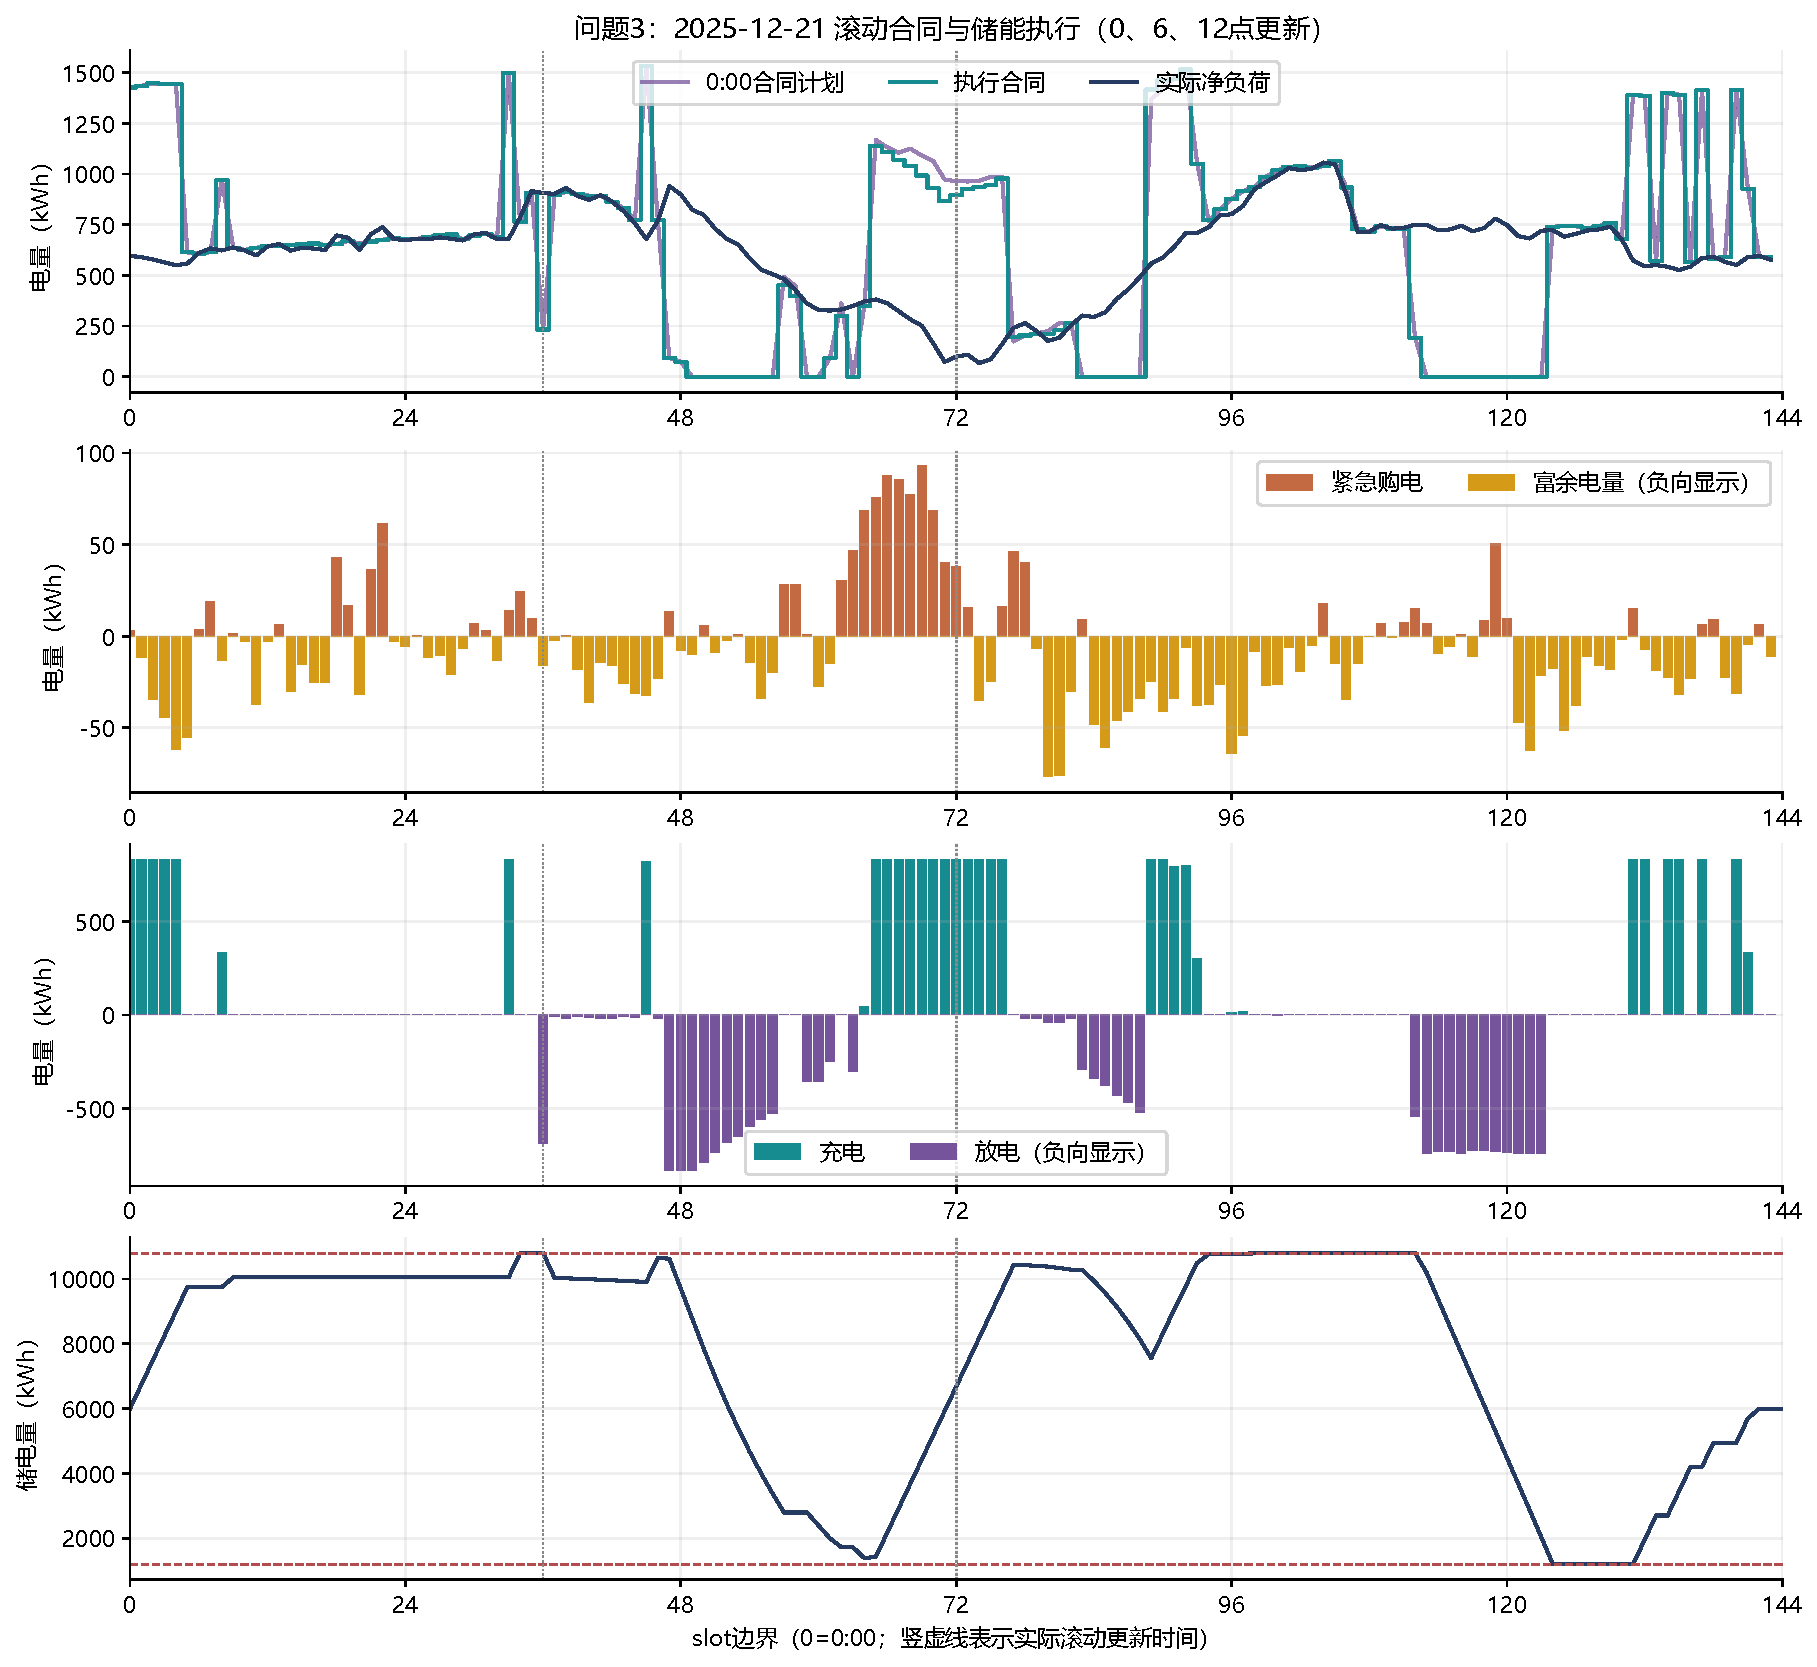
\includegraphics[width=.94\textwidth]{figures/q3_dispatch.pdf}
\caption{12月21日三时刻策略执行轨迹，6点和12点后仅调整未执行部分}\end{figure}
\subsection{预报时刻的经济价值}

\begin{table}[H]\centering\small
\caption{中点插值下六种预报组合的334天回测}
\begin{tabular}{lrrr}\toprule
预报组合 & 总费用/元 & 紧急电量/kWh & 相对仅0点节省/元\\\midrule
0 & 17365850.5168 & 380700.5461 & 0.0000\\
0+6 & 17102438.5627 & 300935.5745 & 263411.9541\\
0+6+12 & 17020306.6465 & 282085.6383 & 345543.8702\\
0+6+12+18 & 17020342.9202 & 282112.5626 & 345507.5965\\
0+12+18 & 17109577.9735 & 321945.8997 & 256272.5433\\
0+6+18 & 17102086.8102 & 300951.5733 & 263763.7066\\
\bottomrule\end{tabular}\end{table}
沿0点、加入6点、再加入12点的顺序，费用分别减少263411.9541元和82131.9161元。进一步加入18点增加36.2737元。由四时刻集合删除6点和12点，分别增加89235.0532元和81743.8900元。因此当前回测支持保留6点、12点。
18点的费用变化相对于全期费用极小，应表述为“本次回测未见额外经济收益”，不应认为18点预报普遍无用。六种组合未穷举所有子集，且策略在同年回测中比较并选择，仍需独立验证期判断泛化效果。
\subsection{共同窗口预测误差与离散稳健性}
用MAE与RMSE评价光伏功率预报，避免夜间真值为零时MAPE失真。不同发布时间的剩余窗口长度不同，不能直接把RMSE下降全部归因于预报更新。固定18:00--24:00共同窗口后，各组均使用12024个样本。

\begin{table}[H]\centering\small
\caption{不同预报的功率误差（kW）}
\begin{tabular}{lrrr}\toprule
发布时间 & 剩余窗口样本数 & 剩余RMSE & 共同窗口RMSE\\\midrule
0:00 & 48096 & 388.7783 & 62.7411\\
6:00 & 36072 & 286.8708 & 60.7876\\
12:00 & 24048 & 166.1577 & 60.5573\\
18:00 & 12024 & 60.0726 & 60.0726\\
\bottomrule\end{tabular}\end{table}
12点到18点在共同窗口的RMSE仅改善0.4847 kW。误差更小不保证合同调整与紧急费用之和更低，经济价值仍需通过完整执行评价。

\begin{figure}[H]\centering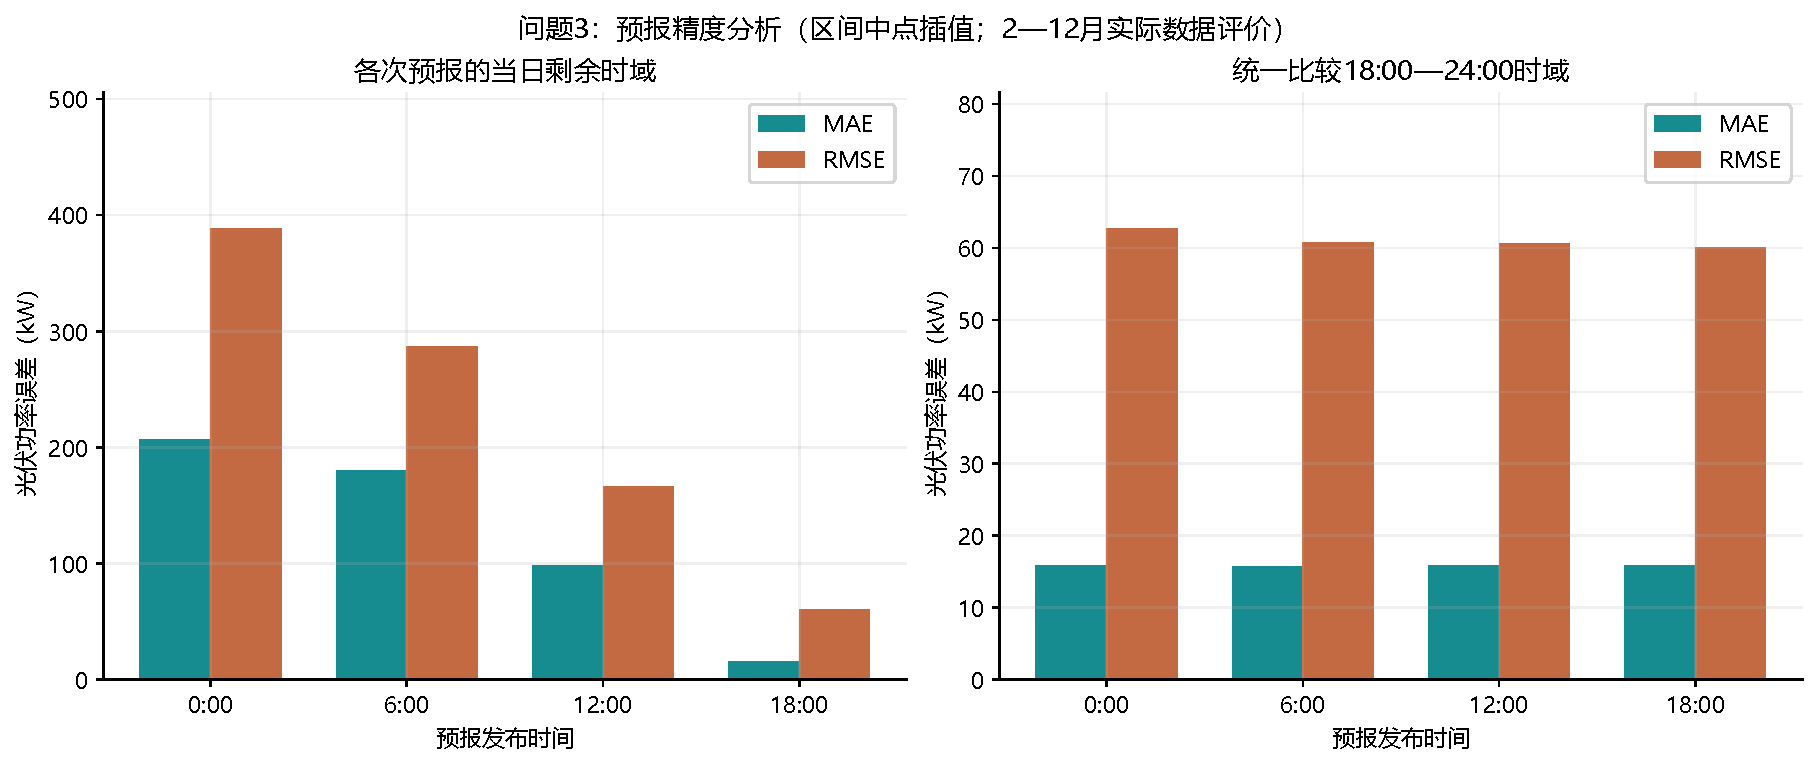
\includegraphics[width=.94\textwidth]{figures/q3_accuracy.pdf}
\caption{预报误差比较：剩余窗口与共同晚间窗口分别统计}\end{figure}
作为离散口径对照，既有端点三时刻实现的费用为17013832.1962元，比中点实现低6474.4504元，约0.0380\%。该差异同时受到采样与数值实现影响，不能证明端点插值普遍更好。两种实现均支持当前三时刻选择；本文主结果、第四问和算法对照统一采用中点实现，端点结果只作为稳健性补充。
\subsection{全期结果与收益分解}

\begin{table}[H]\centering\small
\caption{问题三：334天正式主策略汇总}
\begin{tabular}{lr}\toprule
指标 & 数值\\\midrule
初始合同量/kWh & 25627255.4413\\
执行合同量/kWh & 24999199.3025\\
紧急购电量/kWh & 282085.6383\\
实际总购电量/kWh & 25281284.9407\\
初始计划费/元 & 15933478.6262\\
调整净费/元 & 9377.4177\\
紧急费/元 & 1077450.6027\\
实际总费/元 & 17020306.6465\\
\bottomrule\end{tabular}\end{table}
相对问题二，费用减少589485.0400元，降幅3.3475\%；紧急电量减少40.9178\%。其中由问题二到仅0点预报节省243941.1698元，再引入6点、12点滚动更新节省345543.8702元。这区分了初始预报信息与日内调整的收益，不能把全部差异归因于滚动控制。仍有243天发生紧急补购，说明策略减少费用和补购规模，并未消除预测偏差。
\FloatBarrier
